\documentclass{article}
\usepackage[utf8]{inputenc}

\title{CS246 Homework 1 Answers}
\author{Charlie Zhang}
\date{Jan 2013}

\usepackage{natbib}
\usepackage{graphicx}
\linespread{1.3}

\begin{document}

\maketitle
\section{Problem Set 1}

Friend recommendations:

924 ---- 6995,43748,45881,11860,15416,439,2409

8941 ---- 8938,8942,8946,8945,8944,8939,8943,8940

8942 ---- 8941,8939,8938,8946,8945,8940,8944,8943

9019 ---- 320,9018,9020,9021,9022,9017,9016,9023,317

9020 ---- 9021,9022,9019,9018,320,9017,9016,9023,317

9021 ---- 9020,9022,9019,9018,320,9017,9016,9023,317

9022 ---- 9020,9021,9019,9023,317,320,9018,9017,9016

9990 ---- 9994,9993,9987,9988,9989,35667,9991,9992,34642,37941

9992 ---- 9987,9989,9994,9993,35667,9988,9990,9991

9993 ---- 9994,9990,9991,9987,9988,9989,35667,9992,34642,37941


\section{Problem Set 2}
\subsection{(a)}

A drawback of using confidence is that it ignores P (B). Why is this a drawback? Explain
why lift and conviction do not suffer from this drawback?

\textbf{Answer:}

The drawback is that, if B occurs frequently, conf(A $\rightarrow$ B) will always be high no matter what A is. In this case, conf can't describe the importance/interestness of association A $\rightarrow$ B.

lift avoids this drawback by using S(B) as a denominator, if B occurs frequently, life(A $\rightarrow$ B) will reduce.
conv does not suffer from this drawback since it compares the cases where B is not present.


\subsection{(b)}

A measure is symmetrical if measure(A $\rightarrow$ B) = measure(B $\rightarrow$ A). Are all the measures
presented here symmetrical? Explain.

\textbf{Answer:}

conf is not symmetrical:

$conf(A \rightarrow B) = P(B | A) = \frac{S(A \cap B)}{S(A)}$

$conf(B \rightarrow A) = P(A | B) = \frac{S(A \cap B)}{S(B)}$


lift is symmetrical:

$lift(A \rightarrow B) = \frac{conf(A \rightarrow B)}{S(B)} = \frac{S(A \cap B)}{S(A) * S(B)}$

$lift(B \rightarrow A) = \frac{conf(B \rightarrow A)}{S(A)} = \frac{S(A \cap B)}{S(B) * S(A)}$


conv is not symmetrical:

$conv(A \rightarrow B) = \frac{(1 - S(B))}{(1 - conf(A \rightarrow B))} = \frac{(1 - S(B))}{(1 - \frac{S(A \cap B)}{S(A)})} \ne \frac{(1 - S(A))}{(1 - \frac{S(A \cap B)}{S(B)})}$



\subsection{(c)}

A measure is desirable if its value is maximal for rules that hold 100\% of the time (such rules
are called perfect implications). This makes it easy to identify the best rules. Which of the
above measures have this property? Explain why.

\textbf{Answer:}

They're all desirable.

since $S(A \cap B) \le S(A)$, and $S(A \cap B) = S(B)$ only when the rule $A \rightarrow B$ holds 100\% of time.

conf reaches maximal of 1 when  $S(A \cap B) = S(B)$

life reaches maximal of $\frac{1}{S(B)}$ when  $S(A \cap B) = S(B)$

conv reaches maximal of a infinite value when  $S(A \cap B) = S(B)$




\subsection{(d)}

List the top 5 rules in decreasing order of confidence score for itemsets of size 2. Do it also
for itemsets of size 3. (Ties can be broken arbitrarily.)

\textbf{Answer:}

Top 5 rules by "conf" score (itemsize=2):

('DAI93865',) $\rightarrow$ ('FRO40251',), 1.000000

('GRO85051',) $\rightarrow$ ('FRO40251',), 0.999176

('GRO38636',) $\rightarrow$ ('FRO40251',), 0.990654

('ELE12951',) $\rightarrow$ ('FRO40251',), 0.990566

('DAI88079',) $\rightarrow$ ('FRO40251',), 0.986726


Top 5 rules by "conf" score (itemsize=3):

('DAI31081', 'GRO85051') $\rightarrow$ ('FRO40251',), 1.000000

('ELE26917', 'GRO85051') $\rightarrow$ ('FRO40251',), 1.000000

('GRO85051', 'SNA80324') $\rightarrow$ ('FRO40251',), 1.000000

('ELE20847', 'FRO92469') $\rightarrow$ ('FRO40251',), 1.000000

('GRO73461', 'GRO85051') $\rightarrow$ ('FRO40251',), 1.000000


\subsection{(e)}

List the top 5 rules in decreasing order of lift score for itemsets of size 2. Do it also for
itemsets of size 3. (Ties can be broken arbitrarily.)

\textbf{Answer:}

Top 5 rules by "lift" score (itemsize=2):

('SNA44451',) $\rightarrow$ ('DAI18527',), 67.641876

('SNA82528',) $\rightarrow$ ('DAI43868',), 50.945127

('FRO17734',) $\rightarrow$ ('ELE28189',), 50.104399

('GRO30912',) $\rightarrow$ ('ELE88583',), 47.411585

('GRO89004',) $\rightarrow$ ('ELE25077',), 45.420108


Top 5 rules by "lift" score (itemsize=3):

('FRO19221', 'SNA93860') $\rightarrow$ ('SNA53220',), 40.484449

('DAI62779', 'DAI92600') $\rightarrow$ ('DAI42083',), 35.345477

('DAI92600', 'ELE17451') $\rightarrow$ ('DAI42083',), 34.172245

('DAI85309', 'ELE92920') $\rightarrow$ ('SNA18336',), 30.336175

('DAI42083', 'DAI62779') $\rightarrow$ ('DAI92600',), 29.852461


\subsection{(f)}

List the top 5 rules in decreasing order of conviction score for itemsets of size 2. Do it also
for itemsets of size 3. (Ties can be broken arbitrarily.)

\textbf{Answer:}

Top 5 rules by "conv" score (itemsize=2):

('DAI93865',) $\rightarrow$ ('FRO40251',), INF

('GRO85051',) $\rightarrow$ ('FRO40251',), 1062.512182

('GRO38636',) $\rightarrow$ ('FRO40251',), 93.648212

('ELE12951',) $\rightarrow$ ('FRO40251',), 92.772995

('DAI88079',) $\rightarrow$ ('FRO40251',), 65.933011


Top 5 rules by "conv" score (itemsize=3):

('DAI31081', 'GRO85051') $\rightarrow$ ('FRO40251',), INF

('ELE26917', 'GRO85051') $\rightarrow$ ('FRO40251',), INF

('GRO85051', 'SNA80324') $\rightarrow$ ('FRO40251',), INF

('ELE20847', 'FRO92469') $\rightarrow$ ('FRO40251',), INF

('GRO73461', 'GRO85051') $\rightarrow$ ('FRO40251',), INF



\subsection{(g)}

From all the sets of rules you found in parts (d), (e) and (f), list all the rules (for itemsets
of size 2) which hold 100\% of the time (maximal for perfect implications)? Hint: Apply
concepts from part (c).

\textbf{Answer:}

The rule is: ('DAI93865',) $\rightarrow$ ('FRO40251',),

\subsection{(h)}

Which products would you recommend online on the page for product GRO85051? State
which measure and rule you used for your recommendation.

\textbf{Answer:}

('GRO85051',) $\rightarrow$ ('FRO40251',), conf score 0.999176

('GRO85051',) $\rightarrow$ ('FRO40251',), lift score 8.007055

('GRO85051',) $\rightarrow$ ('FRO40251',), conv score 1062.512182


\subsection{(i)}

Which products would you recommend if we know that the customer has browsed the follow-
ing products: ELE17451, DAI92600, GRO85051? Does your recommendation change if
a different measure is used?

\textbf{Answer:}

I would recommend DAI42083  based on the rule:

('DAI92600', 'ELE17451') $\rightarrow$ ('DAI42083',), lift: 34.171146

('DAI92600', 'ELE17451') $\rightarrow$ ('DAI42083',), conf: 0.573529


If use confidence score as the primary measure, the recommended product would be FRO40251 instead:

('ELE17451', 'GRO85051') $\rightarrow$ ('FRO40251',), conf: 1.000000

('ELE17451', 'GRO85051') $\rightarrow$ ('FRO40251',), lift: 8.013656


\subsection{(j)}

Retailers commonly offer deals at the checkout counter at the store. The counter clerks are
only able to suggest one or two recommendations. Which products would you recommend
to a customer at the checkout counter if the customer has the following products in the cart:
ELE92920, DAI93865, DAI88079, DAI23334? Would you make your recommendations
based on 2- or 3-itemsets? Explain which would you choose and why.

\textbf{Answer:}

I would recommend DAI42083, FRO40251 and DAI62779 based on the rules below:

('DAI92600', 'ELE17451') $\rightarrow$ ('DAI42083',), conv: 2.305472

('DAI92600', 'ELE17451') $\rightarrow$ ('DAI42083',), conf: 0.573529

('DAI92600', 'ELE17451') $\rightarrow$ ('DAI42083',), lift: 34.171146


('ELE17451', 'GRO85051') $\rightarrow$ ('FRO40251',), conv: 875212943.243217

('ELE17451', 'GRO85051') $\rightarrow$ ('FRO40251',), conf: 1.000000

('ELE17451', 'GRO85051') $\rightarrow$ ('FRO40251',), lift: 8.013656


('DAI23334', 'ELE92920') $\rightarrow$ ('DAI62779',), conf: 1.000000

('DAI23334', 'ELE92920') $\rightarrow$ ('DAI62779',), conv: 785633837.443231

('DAI23334', 'ELE92920') $\rightarrow$ ('DAI62779',), lift: 4.664917


I made my recommendations based on 3-itemsets as they give more precise recommendations than 2-itemsets.


\section{Problem Set 3}

\subsection{(a) Necessary Condition}

For a similarity function sim to have a locality sensitive hashing scheme of the form given
above, prove that the function $d(x, y) = 1 - sim(x, y)$ has to satisfy the triangle inequality.
 ($d(x, y) + d(y, z) \ge d(x, z)$, for all $x, y, z.$)

\textbf{Answer:}

Suppose we have x, y, z where $d(x, y) + d(y, z) < d(x, z)$ and the similarity function is a locality sensitive hashing, i.e, $sim(x, y) = Pr[x = y]$.

Then:

$d(x, y) + d(y, z) < d(x, z)$

$1 - sim(x, y) + 1 - sim(y, z) < 1 - sim(x, z)$

$sim(x, y) + sim(y, z) - sim(x, z) > 1$

$Pr[x = y] + Pr[y = z] - Pr[x = z] > 1$

$Pr[x = y\;OR\;y = z] - (Pr[x = z] - Pr[x = y\;AND\;y = z]) > 1$

$Pr[x = y\;OR\;y = z] > 1$ is impossible. Such locality sensitive hashing scheme doesn't exist.

So $d(x, y) = 1 - sim(x, y)$ has to satisfy the triangle inequality.

\subsection{(b)}

\textbf{Answer:}

Counter Example: 

$A = {1}, B = {1, 2}, C = {2}$

$Sim(A, B) = 1, Sim(B, C) = 1, Sim(A, C) = 0$

$Pr[h(A) = h(B)] = 1, Pr[h(B) = h(C)] = 1, Pr[h(A) = h(C)] = 0$

Since $Pr[h(A) = h(B)] = 1, Pr[h(B) = h(C)] = 1$, $Pr[h(A) = h(C)] = 1$ must be 1, which is contrary to the similarity defined by the function.


\subsection{(c)}

\textbf{Answer:}

Counter Example: 

$A = {1}, B = {1, 2}, C = {2}$

$Sim(A, B) = 2/3, Sim(B, C) = 2/3, Sim(A, C) = 0$

$Pr[h(A) = h(B)] = 2/3, Pr[h(B) = h(C)] = 2/3, Pr[h(A) = h(C)] = 0$

We can conclude that:

$Pr[h(A) = h(B)\;OR\;h(B) = h(C)] = 4/3 - Pr[h(A) = h(B)\;AND\;h(B) = h(C)] = 4/3 > 1.$

Which is impossible.


\section{Problem Set 4}

\subsection{(a)}
Let's define a random variable X as $\sum\nolimits_{j=1}^L |T \cap Wj|$

$Exp(X) = L * n(T) * Pr[x = z | x \in T ] < L * n * p2^k = L * n * p2^{\log_\frac{1}{p2} n} = L$

Based on Markov's Inequality, $Pr[X > 3L] < \frac{Exp(X)}{3L} = \frac{1}{3}$.

\subsection{(b)}

For given j, $Pr[g_j(x*) = g_j(z)] \ge p1^k = p1^{\log_\frac{1}{p2} n} = n^{-\rho}$

$l = n^{\rho}$,

$Pr[j \in [1:L] g_j(x*) \ne g_j(z)] \le (1 - Pr[g_j(x*) = g_j(z)])^L = (1 - n^{-\rho})^{n^{\rho}} <= \frac{1}{e}$

\subsection{(c)}

Let's define

E1: The returned point is an actual $(c,\lambda)$-ANN

E2: Total number of false positive points (points that has $D \ge c\lambda$) is less than 3L

E3: An actuall $(c,\lambda)$-ANN is retrieved from at lease one of the buckets

Based on previous results, we have $Pr[E1] > \frac{2}{3}$, and $Pr[E2] > \frac{1}{e}$

$Pr[E1] = Pr[E2] * Pr[E3] > \frac{2}{3e}$


\subsection{(d)}

The total execution time for 10 rounds of LSH lookup: 0.104638 seconds.

The total execution time for 10 rounds of linear search: 1.618231 seconds.

error = 1.1034

\begin{figure}
\centering
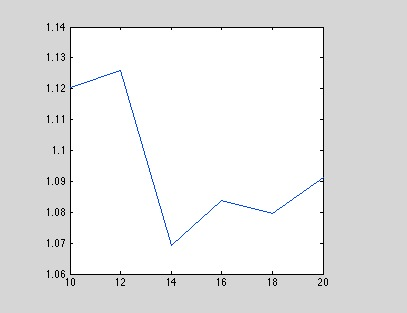
\includegraphics[scale=0.5]{lsh/errs_l.png}
\caption{Error as a function of dirrerent L values}
\label{threadsVsSync}
\end{figure}

\begin{figure}
\centering
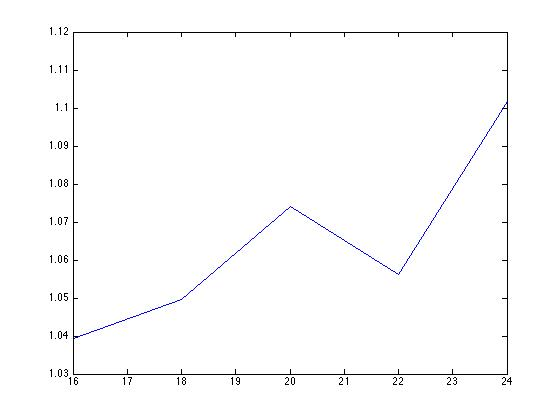
\includegraphics[scale=0.5]{lsh/errs_k.jpg}
\caption{Error as a function of dirrerent k values}
\label{threadsVsSync}
\end{figure}

\begin{figure}
\centering
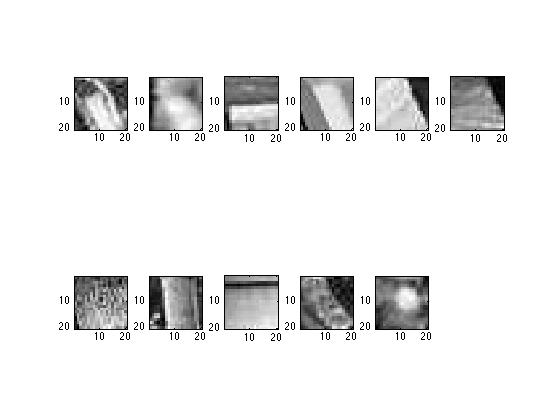
\includegraphics[scale=0.5]{lsh/neighbours_of_100_by_lsh.jpg}
\caption{Top 10 neighbours of patch 100 by LSH}
\label{threadsVsSync}
\end{figure}

\begin{figure}
\centering
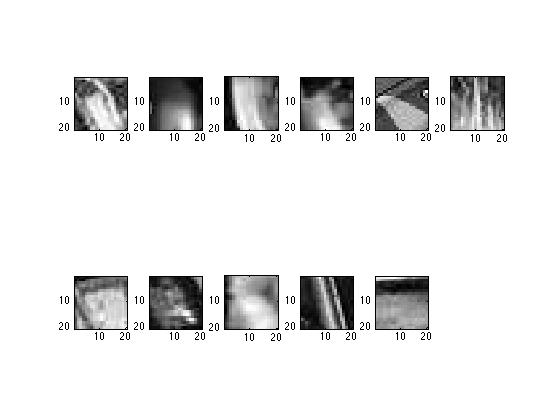
\includegraphics[scale=0.5]{lsh/neighours_of_100_by_linear_search.jpg}
\caption{Top 10 neighbours of patch 100 by Linear search}
\label{threadsVsSync}
\end{figure}

Visually linear search results look more similar to the original picture.

\end{document}
